\section{Experimental Results}\label{sec:results}

In this section we discuss our experimental evaluation of the work profiling strategies and
the effectiveness of the work efficiency metric on guiding true online {\itercomp}.
We use the following naming convention for the profiling strategies considered
throughout this section:
\begin{itemize}[leftmargin=3mm]
\item \textbf{\OracleRM} measures the actual speedup over the unoptimized version of the program for any given input. In our experiments,
    this oracle is allowed to execute each input \emph{at least twice} so the speedup can be computed.
\item \textbf{\OraclePP} measures the work efficiency metric with a \textit{magically perfect} non-intrusive profiling.
  Because this version simulates a \textit{perfect} profiling, with zero overhead,
  it allows us to isolate and evaluate the actual effectiveness of the work efficiency metric.
\item \textbf{\OptProf} corresponds to the work profiling using the optimal placement of the probes. This profiling strategy requires
    \emph{a single execution} of the program for any given input.
\item \textbf{\WCRelax-\textit{N}\%} measures the work efficiency metric using the work profiling with a \textit{N}\% threshold for
the \WCRelaxLower relaxation.
  Similar to the \OptProf, this profiling strategy also requires a single execution of the program for any given input.
\item \textbf{\WPRelax-\textit{N}\%} is similar to the \WCRelax, but it applies the \WPRelaxLower relaxation instead.
\end{itemize}

\begin{figure*}[t!]
    \centering
    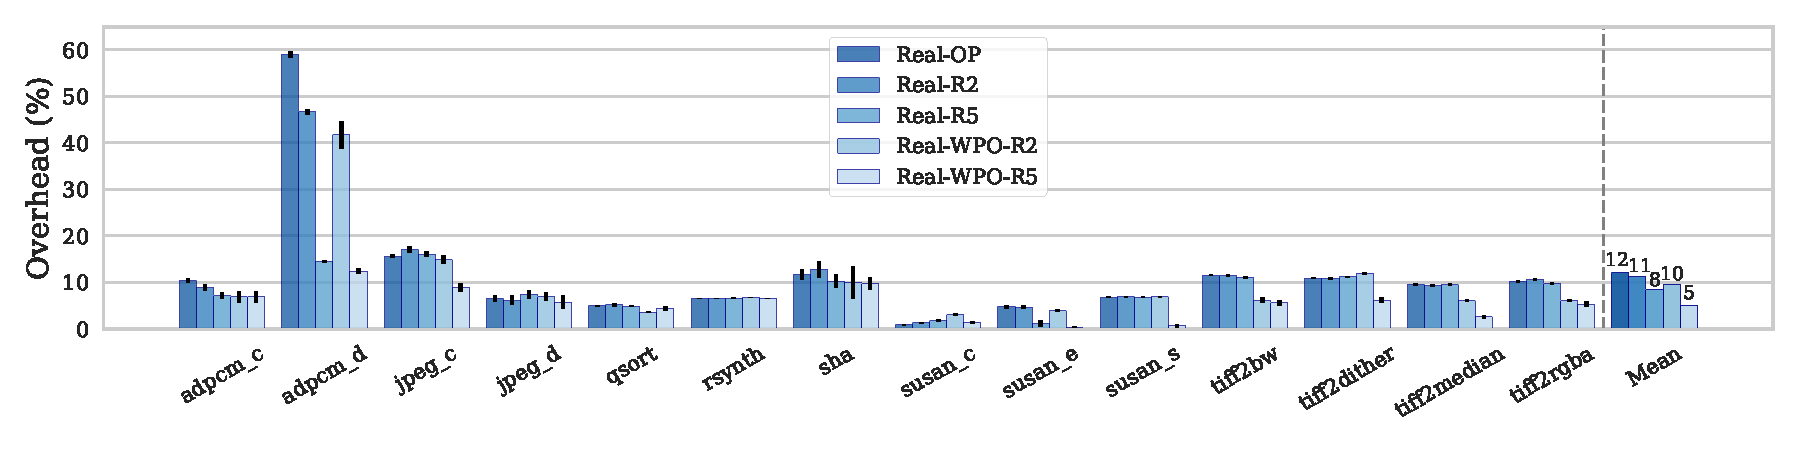
\includegraphics[width=\textwidth]{figs/overhead-O3.pdf}
    \caption{Instrumentation overhead for each benchmark averaged over all inputs, when compiled with {\flagstype -O3}.}
    \vspace{-3mm}
    \label{fig:overhead-O3}
\end{figure*}

\begin{figure*}[t!]
    \centering
    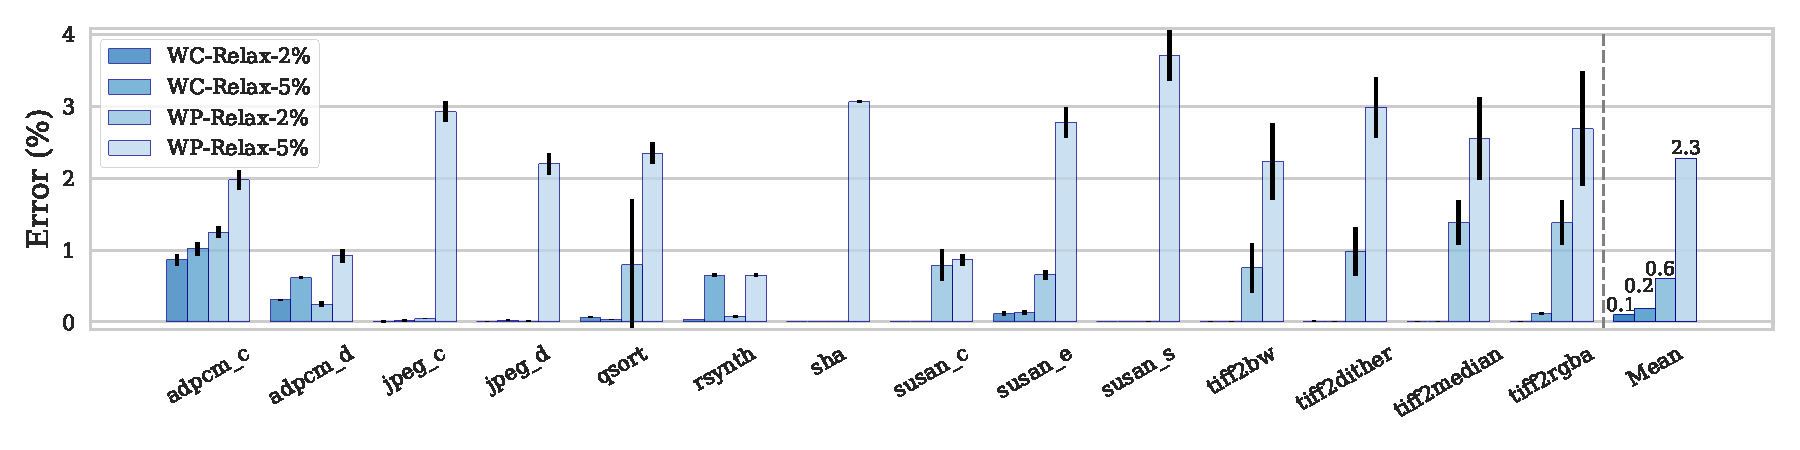
\includegraphics[width=\textwidth]{figs/error-O3.pdf}
    \caption{Dynamic error of the work profiling averaged over the 1000 inputs, after relaxing the number of probes.}
    \vspace{-3mm}
    \label{fig:error-O3}
\end{figure*}

\subsection{Evaluation of the Instrumentation}

First, we evaluate the runtime overhead introduced by the work efficiency profiling. A high overhead would impact the user's experience
and would make our approach impractical. We take the original and instrumented versions of each benchmark, we compile them using the
baseline \texttt{-O3} setting, and execute them with all 1,000 inputs. The difference in their runtimes, for the same input, is the
instrumentation overhead. Figure~\ref{fig:overhead-O3} shows the average overhead for each benchmark and work profiling strategy.

\OptProf typically slows the application down by 10\%, noticeably affecting the user experience, while in the worst case its overhead
reaches 59\%. It is clearly unsuitable for online work profiling. \WCRelax and \WPRelax fare better, especially when used with a higher
5\% threshold. \WPRelax-\textit{5}\%, in particular, has an average overhead of only 5\%, 13\% in its worst case.

For almost all the profiling strategies, their worst case is \texttt{adpcm\_d}. Still, compared to the 59\% overhead of the \OptProf,
\WCRelax-\textit{5}\% and \WPRelax-\textit{5}\% incur only about a quarter of that overhead. This benchmark has a single hot function
consisting mainly of a single hot loop with several branches inside it. Most of the overhead comes from two probes which are placed in
very frequently executed blocks but contribute little to the total work of the loop. The maximum possible error caused by removing either
of the probes, based on the analysis of the DAG, is about 1.3\%. Both relaxation strategies identify this opportunity and remove the probes.

Some benchmarks display unexpectedly higher overheads under the relaxation strategies. This is counter-intuitive because relaxation only
reduces the number of instrumented probes without changing their placement. By analyzing these cases, we noticed that we could not remove
the most frequently executed probes, so relaxation had little positive impact. At the same time, we removed some probes which were
infrequently executed but were taken into consideration by the LLVM optimization heuristics. In some cases, removed probes caused different
and suboptimal decisions to be made, very slightly increasing the runtime.

Figure~\ref{fig:error-O3} shows that profiling with relaxation incurs very little dynamic error. It also confirms that the \WCRelaxLower
relaxation is overly conservative, while the \WPRelaxLower relaxation achieves a better trade-off. Although the error bound is not
guaranteed by the \WPRelaxLower relaxation, its dynamic error is always below 5\%. For both relaxation strategies the 2\% threshold is too
conservative to be useful. The rest of the paper only evaluates the 5\% threshold.

\subsection{Evaluation of Online {\IterComp}}

\begin{figure*}[t]
    \centering
    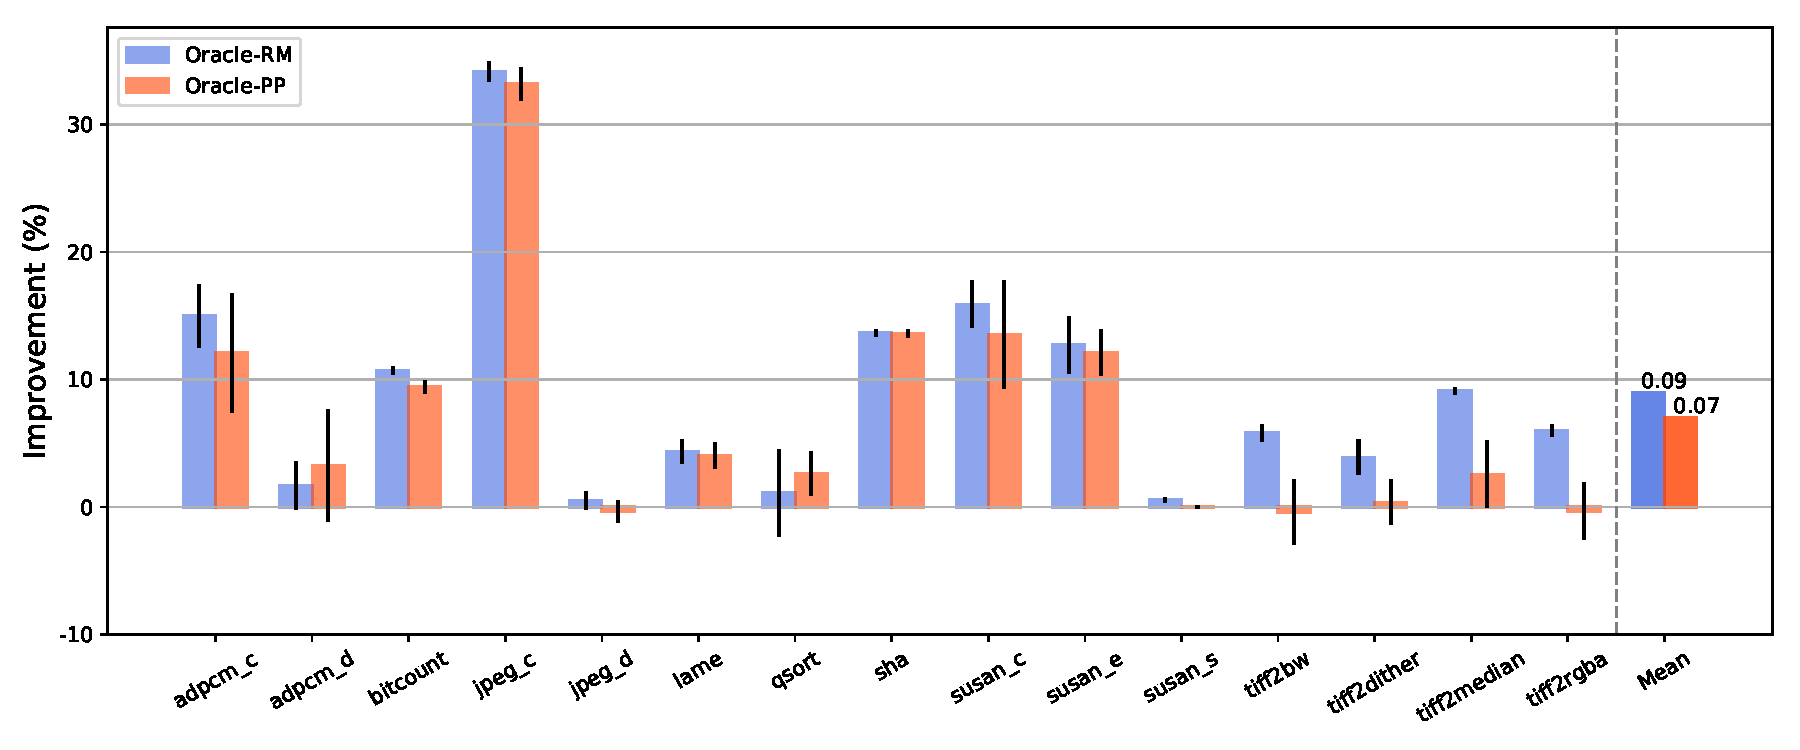
\includegraphics[width=\textwidth]{figs/speedups.pdf}
    \caption{Speedups obtained from the final optimization sequence selected by the online {\itercomp}.
             The speedups reported for each benchmark represents the average speedup across their complete 1000 input datasets.}
    \label{fig:speedups}
\end{figure*}

In this section we evaluate the effectiveness of our work efficiency metric. We perform online {\itercomp} using all five profiling
strategies, namely \OracleRM, \OraclePP, \OptProf, \WCRelax-5\%, and \WPRelax-5\%. We evaluate every optimization sequence on multiple
inputs. We use work efficiency to rank different optimization sequences and we select the one with the highest work efficiency.

\OracleRM makes iterative compilation decisions based on the actual speedup over the unoptimized version. It does not depend on any kind of
instrumentation or work estimation, so it acts as the baseline against which the rest of the profiling strategies are compared. \OraclePP
is also not affected by instrumentation but uses work efficiency instead of speedup. We use it to decide whether our work metric can be
used for iterative compilation on principle. The other configurations demonstrate the viability of applying online {\itercomp} in
real-world scenarios.

We evaluate the quality of the selected optimization sequences by comparing their average speedup over \texttt{-O3} across all 1,000 inputs
of each benchmark.
Figure~\ref{fig:speedups} shows these speedups for all test benchmarks. In most cases, \OraclePP is very close to \OracleRM, achieving on
average 80\% of its speedup. This demonstrates that it is a valid choice to drive iterative compilation decision using work efficiency. The
few cases where the two strategies produce noticeably different results are for the \texttt{tiff} benchmarks. The weaker correlation between
work and unoptimized runtime for these benchmarks is to blame for the lower speedups achieved by \OraclePP.

The \OptProf achieves 4\% improvement on average, which represents a little bit more that half of the speedup of \OraclePP. The culprit is
the one thing that is different between the two strategies, the profiling instrumentation. It affects the search in two key ways:
\textit{(i.)} the overhead incurred by profiling affects the execution time and, through it, the work efficiency metric,
\textit{(ii.)} the inserted instrumentation code occasionally changes how optimizations are applied, e.g., due to the use of a global
variable or in decisions taken based on a cost-model for the instructions. With the \OptProf configuration, instrumentation is very
intrusive and this translates into lower speedups or even slowdowns for five benchmarks. Just measuring work with traditional profiling
approaches is not enough for online iterative compilation.

This is where our two relaxation algorithms become particularly important. Beyond just reducing the user perceived overhead of iterative
compilation, they also improve the search itself by keeping the behavior of the instrumented binary as close as possible to that of the
uninstrumented one. Relaxation reduces the deleterious effects of instrumentation on both the runtime and how optimizations are applied.
As a result, \WCRelax-5\% and \WPRelax-5\% are very close to the behavior of \OraclePP and they achieve about 60\% of the performance
improvement obtained by \OracleRM.

\begin{figure*}[t]
  \centering
  \subfigure[\OptProf]{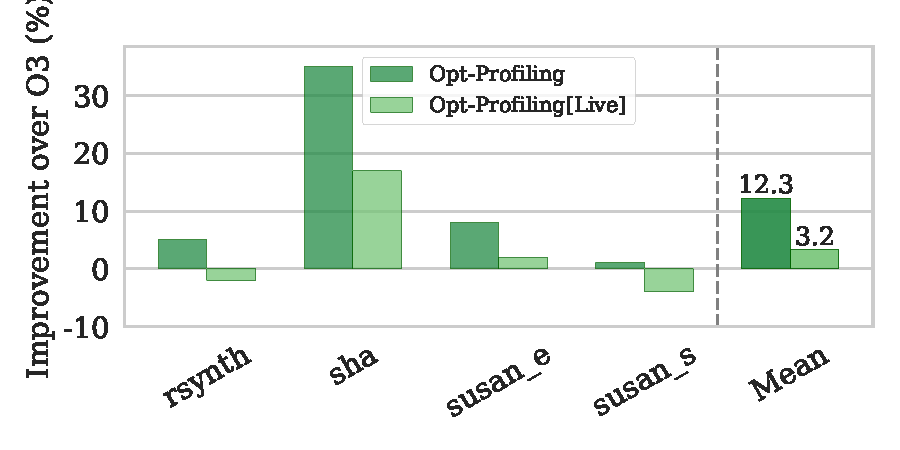
\includegraphics[width=0.3\textwidth]{figs/Opt-Profiling-deployment.pdf}}
  \hfill
  \subfigure[\WCRelax-5\%]{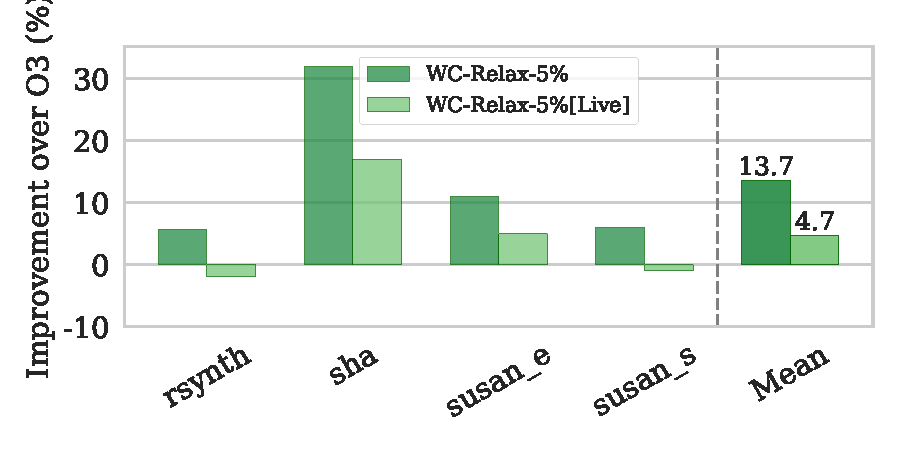
\includegraphics[width=0.3\textwidth]{figs/WC-Relax-5-deployment.pdf}}
  \hfill
  \subfigure[\WPRelax-5\%]{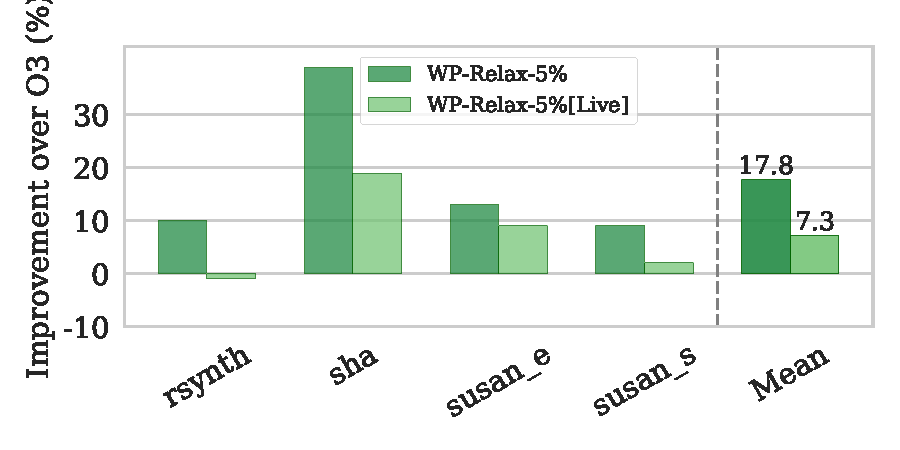
\includegraphics[width=0.3\textwidth]{figs/WP-Relax-5-deployment.pdf}}
  \caption{Speedup over \texttt{-O3} for the best optimization selected by the search, as well as the average speedup as experienced by the
    user throughout the search process ([Live]). The results show that the proposed approach is profitable in real-world online scenarios.}
  \label{fig:deployment_cost}
\end{figure*}

\subsubsection{Cost Evaluation During the Online Search}\label{subsubsec:search}

A typical argument against online adaptive techniques is that the overhead of management and the slowdown due to testing suboptimal
configuration might overshadow the benefits of the technique. In this subsection, we establish that online iterative compilation is
profitable even when factoring in the online costs. We modify the architecture described in Section~\ref{sec:oic-infra} to make it more
realistic by using genetic search~\cite{knijnenburg02,kulkarni04} over the whole space of possible optimizations. 

Figure~\ref{fig:deployment_cost} shows, for each benchmark and configuration, the speedup over \texttt{-O3} of the best optimization sequence
evaluated by the search but also the average profitability/cost experienced by the user throughout the search process (labeled as [Live]),
which takes into account the overhead of the work profiling. We evaluate three configurations that use work profiling, namely \OptProf,
\WCRelax-5\%, and \WPRelax-5\%. By widening the search space, we are able to improve performance significantly compared to the results in
Figure~\ref{fig:speedups}. In terms of the overall speedup throughout the search, all three configurations are profitable on average. 
Although there is a slight risk we select a suboptimal version and the user experiences slowdown, our genetic search focuses on promising
optimization sequences, reducing the risk of selecting a suboptimal version of the program as the genetic population evolves. For all three
configurations, after the first generation, the optimization sequences we evaluate tend to overcome this issue, with their benefits
surpassing the profiling overheads. This is particularly true for \WPRelax-5\%, where the small overhead combined with the large speedup
lead to a 7.3\% overall speedup.
